\documentclass[
	trilingual,
	type=projectproposal,
	twocolumn
]{bfhpub}
% Include Packages
\usepackage[french,ngerman,main=english]{babel}
 
\begin{document}
 
\title{Improving the graphical user interface of Vula}
\subject{Das ist ein Teaser auf dem Titelblatt. Making secure communication more accessible by improving the user experience.}
 
\department{BFH TI}
\titlefooterright{Homepage}
 
\advisor{Prof. Dr. J. Appelbaum}
\coadvisor{Dr. M. Musterman}
\expert{Prof. Dr. J. Appelbaum}
\projectpartner{Vula}
 
%
\projectstartdate{24. Dezember 2000}
\studysubmissiondate{24. Dezember 2000}
\reportsubmissiondate{24. Dezember 2000}
\presentationdate{Prüfungs/Präsentationsdatum}
 
 
\begin{ProjectDescription}
  \section{Projektbeschreibung}
  Students that are enrolled in the course BTI2018-25 have the opportunity to make a contribution to a free software project. They will be contributing to Vula. A Tool that provides its users with a way to securely communicate within a local area network. We have chosen to improve the existing graphical user interface (gui). The current version was built with tkinter by students of BFH in a previous iteration of this course. The goal is not to redo the gui but to expand upon it. Vula can be found via Vula.link or Codeberg.org/vula.
\end{ProjectDescription}
 
\maketitle
 
\section{Projektziele}
\begin{itemize}
  \item Evaluate the current gui
  \item Itemize and prioritize the areas that need improvement.
  \item Come up with solutions to the issues we decide to address
  \item Implement and document the changes
\end{itemize}
Some examples of improvable areas are:
\begin{itemize}
  \item Example 1: Revamp the design of the scrollbars to have a more modern and homogenous look.
  \item Example 2: Reevaluate the chosen color scheme and improving it in terms of usability, accessibility and design.
  \item Example 3: Using our previous experience in web design and use of similar tools to consider changes to the structure of the program.
\end{itemize}
\vfill

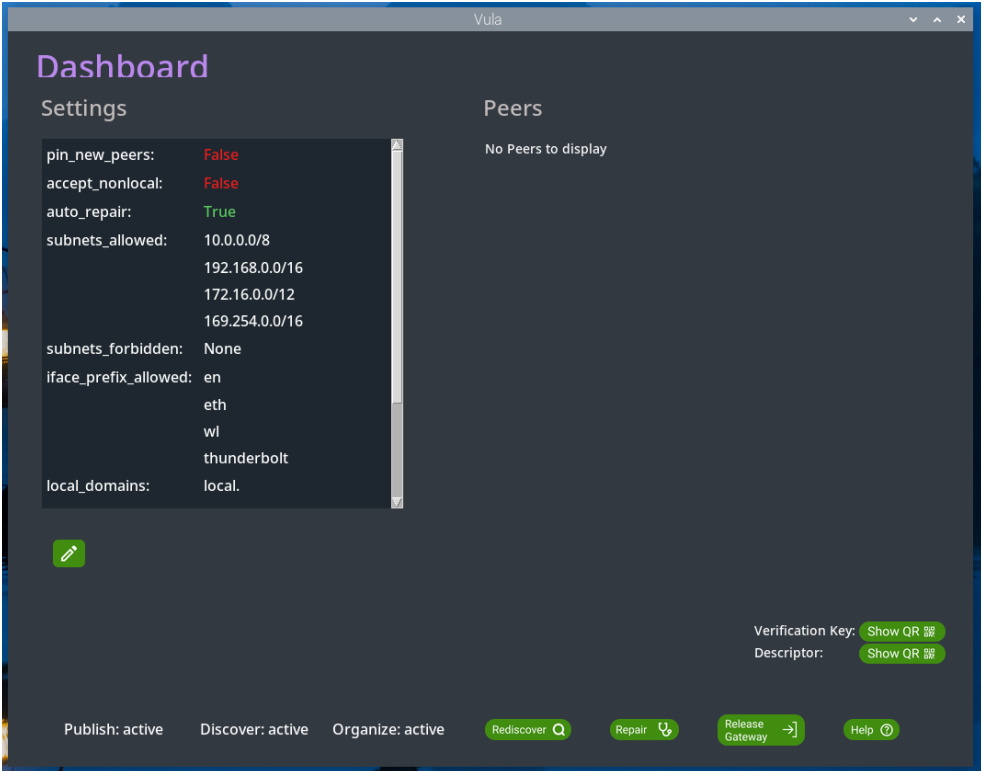
\includegraphics[width=\linewidth]{pictures/dashboard.png}
\par\nointerlineskip\bfhRule
 
\newpage
\begin{thebibliography}{9}
	\bibitem{lamport94}
	Leslie Lamport,
	\textit{\LaTeX: a document preparation system},
	Addison Wesley, Massachusetts,
	2nd edition,
	1994.
\end{thebibliography}
 
\vfill
\DisplayCompetenceRatingChart{
	Experimental=2,
	Mechanical=3,
	Programming=1,
	Electrical=2,
	Conceptual=6
}
 
\end{document}